
%!TEX ROOT=ctutest.tex

\chapter{Rešerše}


\section{Podlahové topení}

U podlahového vytápění dochází k přenosu tepla do vytápěného prostoru převážně sáláním. Což má za následek, že se od sálající plochy ohřívají plochy osálané a teprve od sálajících a osálaných ploch se ohřívá okolní vzduch (druhá konvenkční složka z celkového tepelného toku). Naproti tomu při přenosu tepla pomocí tradičních radiátorů dochází k přenosu pomocí proudění (konvekční složka). 
Teplota otopné plochy je poměrně nízká pohybuje se mezi 25 až 34 °C u podlahového vytápění a tedy i teplota teplonosné látky je nízká (otopná plocha je zahřívaná buď teplou vodou, teplým vzduchem nebo elektricky). 

Důležitým parametrem pro příjemný pobyt v místnosti je prostorové rozložení teploty, jak ve vertikální tak horizontální rovině. Na vertikální rozložení teplot ve vytápěné místnosti je způsobeno nerovnoměrným přívodem tepla a nerovnoměrným ochlazování jednotlivých stěn místnosti. Vertikální nerovnoměrnost teplot je tím větší, čím vyšší je povrchová teplota otopné plochy. Vzhledem k tomu, že teplota u podlahové vytápění je povrchová teplota otopné vody ze všech druhů velkoplošného vytápění (podlahové, stropní, stěnové) nejnižší, je vertikální rozložení teplot skoro ideální. Co se týče rozložení teplot v jednotlivých vrstvách místnosti, je teplota v úrovni hlavy maximálně o 2 až 3 °C vyšší než v oblasti kotníků a směrem od zóny pobytu již klesá. V porovnání s ostatními druhy vytápění je vertikální průběh teplot značně nerovnoměrný. Optimální vytápění by mělo zajistit, aby v oblasti hlavy stojícího člověka byla teplota minimálně o 2 °C nižší než je v úrovni kotníků. Takovému ideálnímu průběhu (obrázek  \ref{fig:vertikalni-prubehy-teplot-pro-ruzne-druhy-vytapeni}a) teplot odpovídá obrázek \ref{fig:vertikalni-prubehy-teplot-pro-ruzne-druhy-vytapeni}b. Dále jsou na obrázku  \ref{fig:vertikalni-prubehy-teplot-pro-ruzne-druhy-vytapeni} jsou další druhy vytápění s vertikálními průběhy teplot.

\begin{figure}[h]
  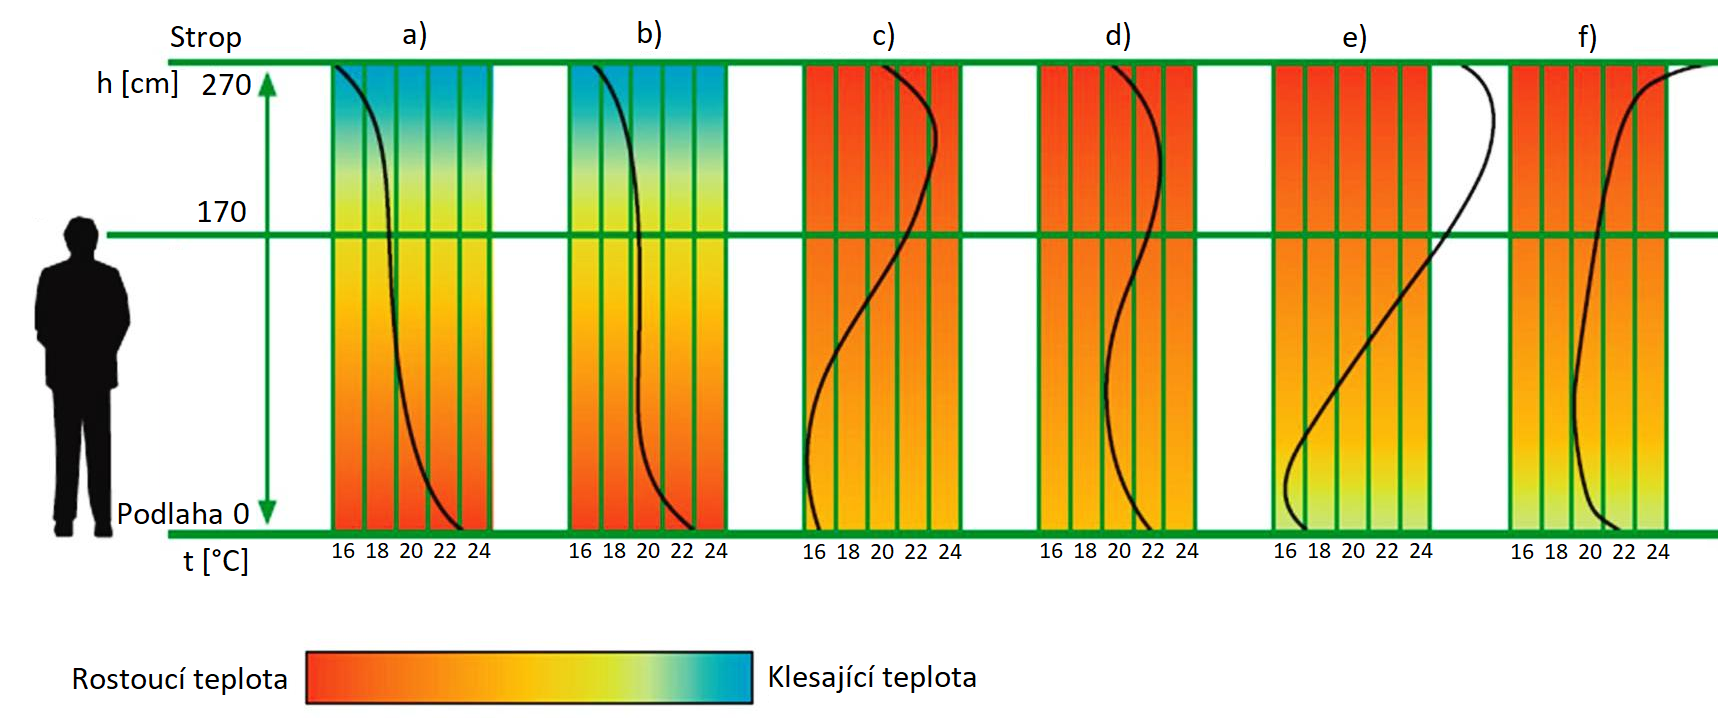
\includegraphics[width=\linewidth]{images/vertikalni-prubehy-teplot-pro-ruzne-druhy-vytapeni.png}
  \caption{Vertikální průběh teploty vzduchu ve vytápěné místnosti při různém způsobu vytápění. \cite{vertikalni-prubehy-teplot-pro-ruzne-druhy-vytapeni} \\ a) Ideální požadovaný průběh, b) Podlahové vytápění, c) Vytápění radiátory (vnitřní stěna), d) Vytápění radiátory (venkovní stěna), e) Teplovzdušné vytápění (podlahové konvektory), f) Stropní vytápění }
  \label{fig:vertikalni-prubehy-teplot-pro-ruzne-druhy-vytapeni}
\end{figure}

Při podlahovém vytápění, teplo postupuje rovnoměrně, plošně a plynule od spodu místnosti, viz obrázek \ref{fig:rozlozeni-teplot-podlahove-vytapeni}. Zatímco tradičnía radiátory ohřívají prostor z jednoho místa a rozložení teplot v místnosti je nerovnoměrné, viz obrázek \ref{fig:rozlozeni-teplot-radiatory}.

\begin{figure}[h]
     \centering
     \begin{subfigure}[b]{0.45\textwidth}
         \centering
         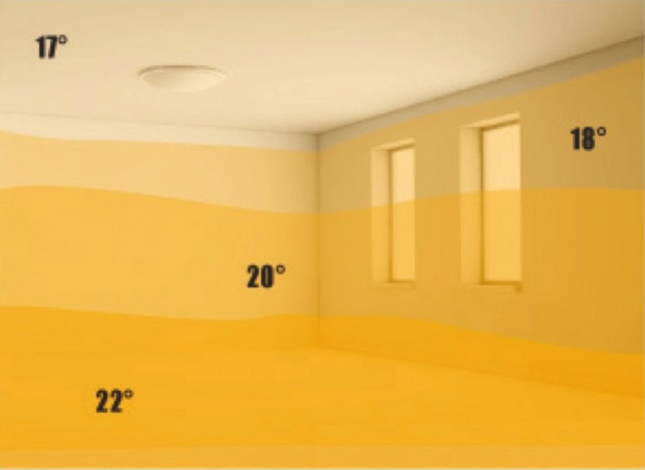
\includegraphics[width=\textwidth]{images/rozlozeni-teplot-podlahove-vytapeni.png}
         \caption{Rozložení teplot při použití podlahové topení.}
         \label{fig:rozlozeni-teplot-podlahove-vytapeni}
     \end{subfigure}
     \hfill
     \begin{subfigure}[b]{0.45\textwidth}
         \centering
         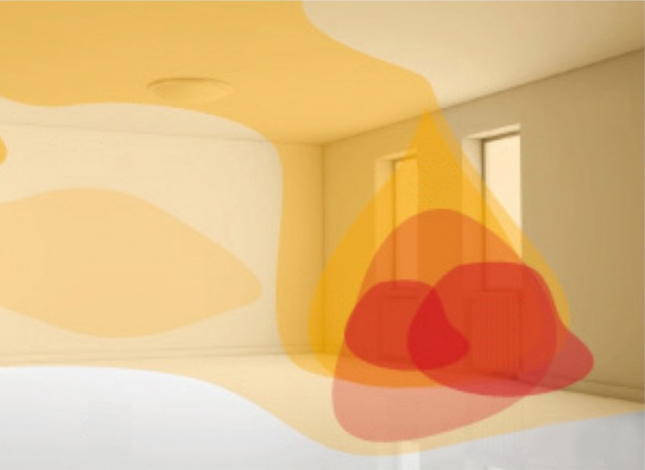
\includegraphics[width=\textwidth]{images/rozlozeni-teplot-radiatory.png}
         \caption{Rozložení teplot při použití radiátorů.}
         \label{fig:rozlozeni-teplot-radiatory}
     \end{subfigure}
\caption{Porovnání rozložení teplot při použití podlahové topení a radiátorů. \cite{rozlozeni-teplot-podlahove-vytapeni-a-radiatory}}
\label{fig:porovnani-rozlozeni-teplot}
\end{figure}

\section{Zónová regulace vytápění}

\subsection{Principy zónové regulace}

\subsection{Dostupné komerční/nekomerční řešení zónové regulace podlahového vytápění}








